%!TEX root = ../dissertation.tex

% Background
\section{Background}
\label{sec:background}

% Service Delivery
\subsection{Related Work}
\label{sub:related work}
As referred in Section~\ref{section:motivation}, current \gls{IoT} solutions are delivered in a physical
and isolated manner, which makes its service delivery model an inefficient and unscalable process.
In order to turn the service delivery of \gls{IoT} solutions more efficient and scalable, cloud service
delivery models are being developed based on the existing layers of the cloud architecture \cite{zhang2010cloud}:
\textit{a) \gls{IaaS}} refers to the provisioning of infrastructure resources on-demand - e.g. \glspl{VM},
storage and network. \textit{b) \gls{PaaS}} refers to providing platform layer resources such as operating
system support and software development frameworks. \textit{c) \gls{SaaS}} refers to providing on demand
application over the Internet.

% Soldatos
\paragraph{Soldatos} et al. \cite{soldatos2012convergence} presented the idea of converging the IoT
and the utility computing in the cloud. The proposed architecture is the core concept of the OpenIoT
Project\footnote{\url{http://openiot.eu}}, and is based on CoAP \cite{shelby2014constrained} and linked data.
The cloud is used at infrastructure level, which allows to measure the utility of the services provided
by inter-connected objects.

% Distefano
\paragraph{Distefano} et al. \cite{distefano2012enabling} proposed a conceptual architecture by
mapping various elements in both cloud and IoT to the three layers of the cloud architecture (\gls{IaaS},
\gls{PaaS} and \gls{SaaS}). In this proposal IoT resources are provided voluntarily by their owners,
while management functions - such as node management and policy enforcement - are viewed as peer
functions of cloud infrastructure management. A \gls{PaaS} module is responsible to mashup IoT and
cloud infrastructure (\gls{IaaS}) resources for applications, which are delivered to the clients
through \gls{SaaS}.

% CloudThings
\paragraph{CloudThings} \cite{zhou2013cloudthings} is an architecture that uses a common
approach to integrate Internet of Things and Cloud Computing. The proposed architecture is an online
platform which accommodates \gls{IaaS}, \gls{PaaS}, \gls{SaaS} and allows system integrators and
solution providers to leverage the complete application infrastructure for developing, operating
and composing applications and services.

% IoT PaaS
\paragraph{Li} et. al \cite{li2013efficient} proposed IoT PaaS, a cloud platform that supports
scalable IoT service delivery. Solution providers are able to deliver new solutions by leveraging
computing resources and platform services - domain mediation, application context management, etc.
- to the cloud. The proposed architecture aims to enable virtual vertical service delivery, for that
it has a multi-tenant nature which is designed to help at the isolation of the environments of
different solutions.\\

Although great progress was achieved regarding the improvement of service delivery for \gls{IoT}
solutions, most of the work still are in a conceptual stage. What is certain is that cloud service
delivery models will be the basis for the service delivery models of \gls{IoT} solutions.

% Data Storage Performance
\subsection{Data Storage Performace}
\label{sub:data_storage}
Since that data storage and retrieval in the cloud had specific requirements, cloud providers started
to implement their own solutions.

\paragraph{Google Big Table, Facebook Cassandra and  Amazon Dynamo} \cite{chang2008bigtable} \cite{lakshman2010cassandra}
\cite{decandia2007dynamo} are key-value stores - \gls{NoSQL} databases - that has the ability to horizontally scale - i.e,
distribute both data and load of simple operations through many servers - but it has a weaker concurrency model
than the ACID transactions of most \glspl{RDBMS} systems \cite{cattell2011scalable}.

\paragraph{\gls{PIQL}} \cite{armbrust2010piql} is a SQL-like API built to run on top of existing
performance predictable key-value stores, that provides many of the benefits of using a traditional
\gls{RDBMS}, such as the ability to express the queries in a declarative way, automatic data
parallelism, physical data independence and automatic index selection and maintenance, all while
maintaining the low latency guarantees on application performance that come from the underlying
key-value store.\\

Recently, some progress has been reached as regards scalable storage for \gls{RDBMS} systems. Although most
of the works still are in development, it is possible to highlight some solutions that are in a more
mature state.

\paragraph{MySQL Cluster} \cite{ronstrom2004mysql} is an in-memory clustered distributed \gls{RDBMS}.
Compared with the MySQL implementation it works by replacing the InnoDB engine with the NDB - a proprietary
distributed layer from MySQL. MySQL Cluster is built on top of a shared-nothing architecture and includes
features such as failover, node recovery, synchronous data replication and no single point of failure.
MySQL Cluster seesm to be the solution that scales to more nodes than other \gls{RDBMS} - 48 is the limit.
However, it was reported that after scaling up to a few dozen nodes it starts to running into
bottlenecks \cite{bunch2010evaluation}.

\paragraph{VoltDB} \cite{stonebraker2013voltdb} is a \gls{RDBMS} designed for performance and scalability.
VoltDB assumes a multi-node cluster architecture where the tables are partitioned over multiple servers.
Tables can be replicated over servers - e.g. for fast access to data - shards are always replicated -
to recovery the data in case of a node crash - and database snapshots are supported. Currently some
features still are missing - online schema changes are limited and asynchronous \gls{WAN} replication and
recovery are not yet implemented - but in its current implementation VoltDB already presents some
features that improves the performance of SQL execution. As result, the number of nodes that are
needed to support a given application load can be reduced in a significant way.

% Fog Computing
\subsection{Fog Computing}
\label{sub:fog_computing}
The Fog Computing \cite{bonomi2012fog} is a platform that aims to bring the cloud close to the ``Edge
of the Network''. By extending the cloud close to the ground, the Fog will be able to meet the requirements
of several applications that the traditional cloud is not able to accomplish. The most notable case
is the Internet of Things, that requires mobility support, geo-distribution in addition to location
awareness and low latency. The Fog achieves that by virtualizing the computing, storage and network
services between end devices and the traditional data centers in the cloud.\\

% Fog Computing Infrastructure
\begin{figure}[ht!]
  \centering
  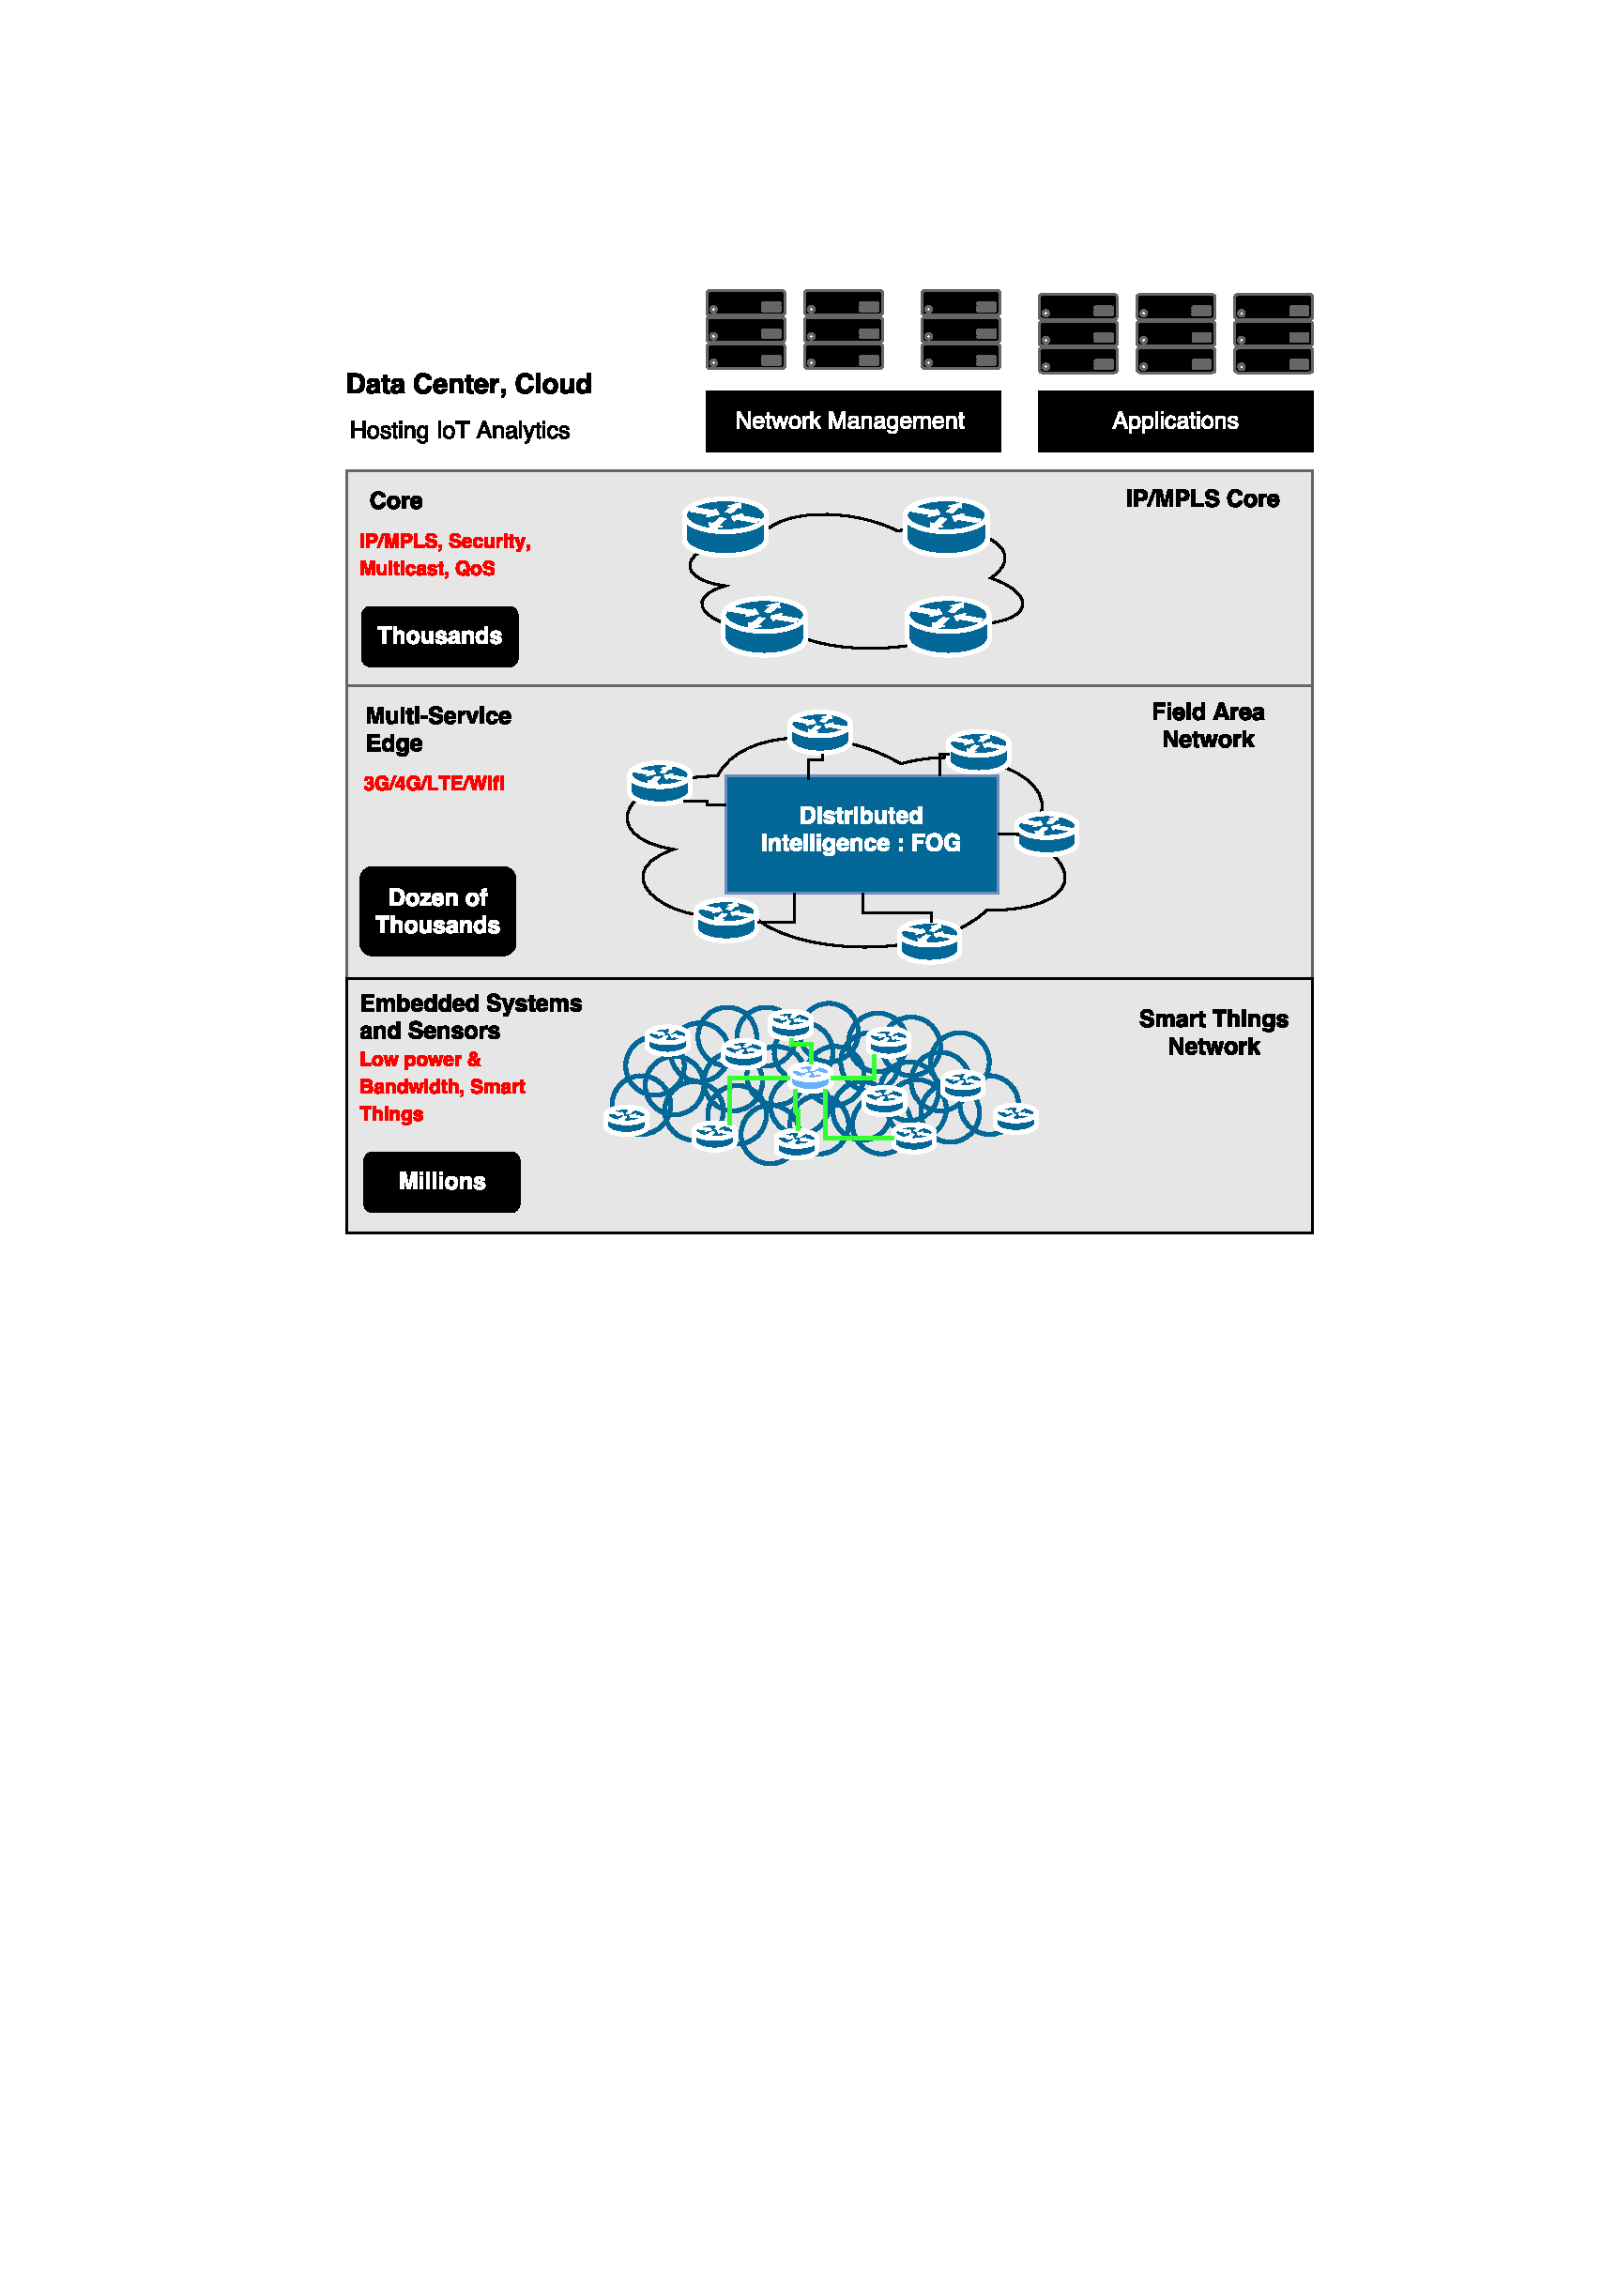
\includegraphics[width=.5\textwidth]{./figures/fog_architecture}
  \caption[IoT and Fog Computing.]{The Internet of Things and Fog Computing (Bonomi et. al (2012)).}
  \label{fig:fog_architecture}
\end{figure}

Figure~\ref{fig:fog_architecture} presents the architecture of the Fog Computing platform.
The distributed infrastructure of the Fog is composed of heterogeneous resources that must be managed
in a distributed way. The infrastructure comprising of several players, covering from data centers,
core of the network, edge of the network and end devices. The \textit{Embedded Systems and Sensors} is
the lowest layer of the Fog and it is responsible to perform \gls{M2M} interaction. It collects and
process the data from the sensors, issues controls to the actuators and also filters the data that
is locally consumed and send the rest to the higher layers. The \textit{Multi-Service Edge} and
\textit{Core} layers are responsible to perform visualization and reporting - e.g. \gls{H2M} interaction -
as well to deal with systems and processes (\gls{M2M}).\\

Since that interaction between the different layers can range from seconds - e.g. low-latency real-time
analytics - to days - transactional analytics - the Fog must support several types of storage, from
ephemeral storage at the lowest layers to semi-permanent at the highest layer. It is important to point
that the higher is the tier, the geographical coverage is wider and the time scale is larger \cite{bonomi2014fog}.
The global coverage is given by the Cloud, which acts as a central repository for the persistent data
and that is used to perform business analytics.

\subsection{RFID Middleware}
\label{sub:rfid_middleware}
The \gls{RFID} middleware is the component of a \gls{RFID} system that sits between the low level
components - e.g. readers and tags - and the business client application - e.g. \gls{ERP} systems.\\

% Fosstrak
\subsubsection{Fosstrak Platform}
\label{subs:fosstrak}
The Free and Open Source Software for Track and Trace (Fosstrak) is an EPCglobal Network compliant
\gls{RFID} software platform that was developed by Floerkemeier et. al \cite{floerkemeier2007rfid}.
Figure~\ref{fig:fosstrak_architecture} presents the architecture of the Fosstrak platform.

% Fosstrak Architecture
\begin{figure}[ht!]
  \centering
  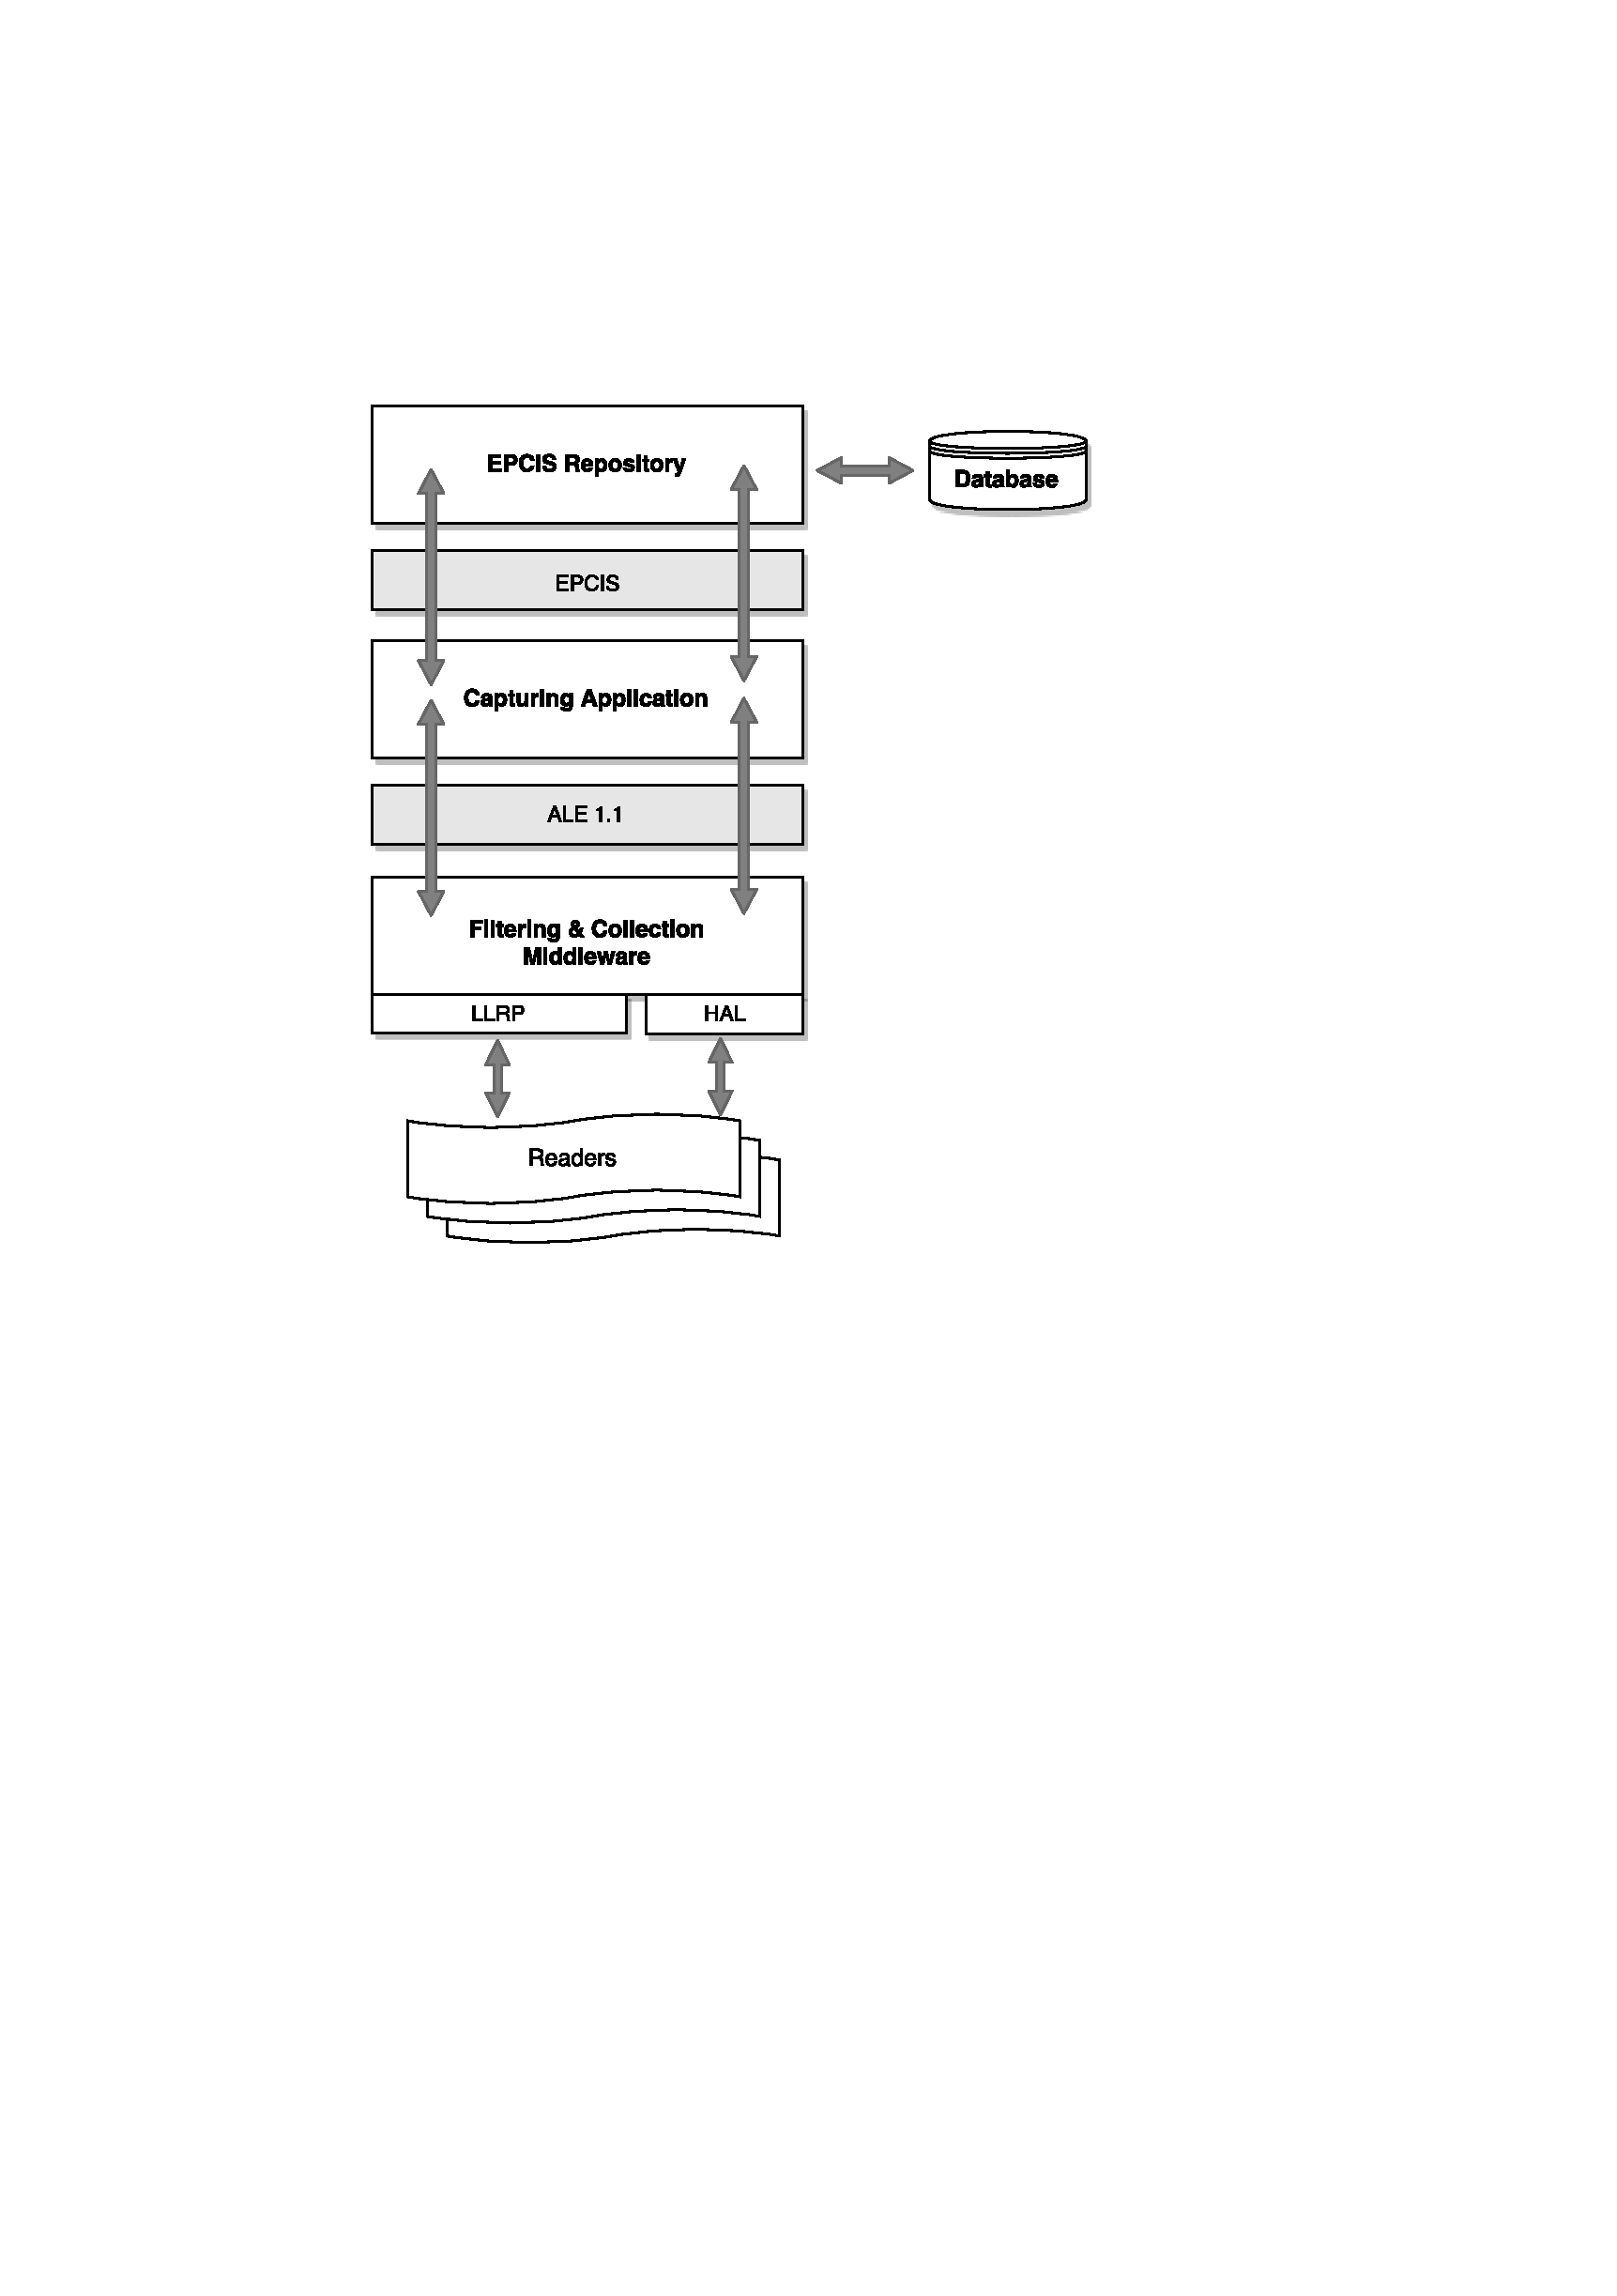
\includegraphics[width=.4\textwidth]{./figures/fosstrak_architecture}
  \caption[Fosstrak architecture.]{Fosstrak architecture.}
  \label{fig:fosstrak_architecture}
\end{figure}

The Fosstrak platform is composed of three modules that implements the corresponding roles in the
\gls{EPC} Network: \textit{Reader Module}, \textit{Filtering and Collection Middleware Module} and
\textit{EPCIS Module}. For our work the relevant modules of the platform are:
% FCServer
\textit{a) Filtering \& Collection Server} is the module responsible to filter and collect data
from \gls{RFID} readers.
% Capturing Application
\textit{b) Capturing Application} is the module responsible to transform the uninterpreted events
into meaningful business events.
% EPCIS Repository
\textit{c) EPCIS Repository} is the module that provides persistence for events.
